\subsection*{Problema 34}
\textbf{Enunciado:} Calcular la integral indefinida
\begin{align*}
\int x^{-1} (4 + 3x^4)^{3/2} \, dx
\end{align*}

\textbf{Solución:} Para resolver la integral, 
utilizamos un cambio de variable adecuado. 
Definimos la sustitución:
\begin{align*}
u &= x^4 \\
du &= 4x^3 \, dx
\end{align*}

Reescribimos la diferencial para 
relacionarla con el integrando. 
Multiplicamos y dividimos por $4x^4$:
\begin{align*}
I &= \int \dfrac{(4 + 3x^4)^{3/2}}{x} \, dx \\
I &= \int \dfrac{(4 + 3x^4)^{3/2} x^3}{4x^4} \, (4x^3 \, dx)
\end{align*}

Sustituyendo $u = x^4$ y $du = 4x^3 \, dx$:
\begin{align*}
I &= \int \dfrac{(4 + 3u)^{3/2}}{4u} \, du \\
I &= \dfrac{1}{4} \int \dfrac{(4 + 3u)^{3/2}}{u} \, du
\end{align*}

Aplicamos un segundo cambio de variable 
para eliminar la potencia fraccionaria. 
Sea $z^2 = 4 + 3u$, de donde $3u = z^2 - 4$ 
y $3 \, du = 2z \, dz$, es decir, 
$du = \dfrac{2}{3}z \, dz$.

Sustituyendo en la integral:
\begin{align*}
I &= \dfrac{1}{4} \int \dfrac{z^3}{\frac{z^2 - 4}{3}} \left(\dfrac{2}{3}z \, dz\right) \\
I &= \dfrac{1}{4} \int \dfrac{3z^3}{z^2 - 4} \left(\dfrac{2}{3}z\right) dz \\
I &= \dfrac{1}{2} \int \dfrac{z^4}{z^2 - 4} \, dz
\end{align*}

Realizamos la división de polinomios 
para el integrando racional:
\begin{align*}
\dfrac{z^4}{z^2 - 4} = z^2 + 4 + \dfrac{16}{z^2 - 4}
\end{align*}

Integramos cada término resultante:
\begin{align*}
I &= \dfrac{1}{2} \int \left( z^2 + 4 + \dfrac{16}{z^2 - 4} \right) dz \\
I &= \dfrac{z^3}{6} + 2z + 4 \int \dfrac{dz}{z^2 - 4}
\end{align*}

Usando fracciones parciales para 
el último término:
\begin{align*}
\int \dfrac{dz}{z^2 - 4} = \dfrac{1}{4} \ln\left| \dfrac{z - 2}{z + 2} \right|
\end{align*}

Combinando los resultados parciales:
\begin{align*}
I = \dfrac{z^3}{6} + 2z + \ln\left| \dfrac{z - 2}{z + 2} \right| + C
\end{align*}

Regresando a la variable original $u$ 
mediante $z = \sqrt{4 + 3u}$:
\begin{align*}
I &= \dfrac{(4+3u)^{3/2}}{6} + 2\sqrt{4+3u} \\
&\quad + \ln\left| \dfrac{\sqrt{4+3u} - 2}{\sqrt{4+3u} + 2} \right| + C
\end{align*}

Finalmente, sustituimos $u = x^4$:
\begin{align*}
I &= \dfrac{(4+3x^4)^{3/2}}{6} + 2\sqrt{4+3x^4} \\
&\quad + \ln\left| \dfrac{\sqrt{4+3x^4} - 2}{\sqrt{4+3x^4} + 2} \right| + C
\end{align*}

\begin{figure}[H]
	\centering
	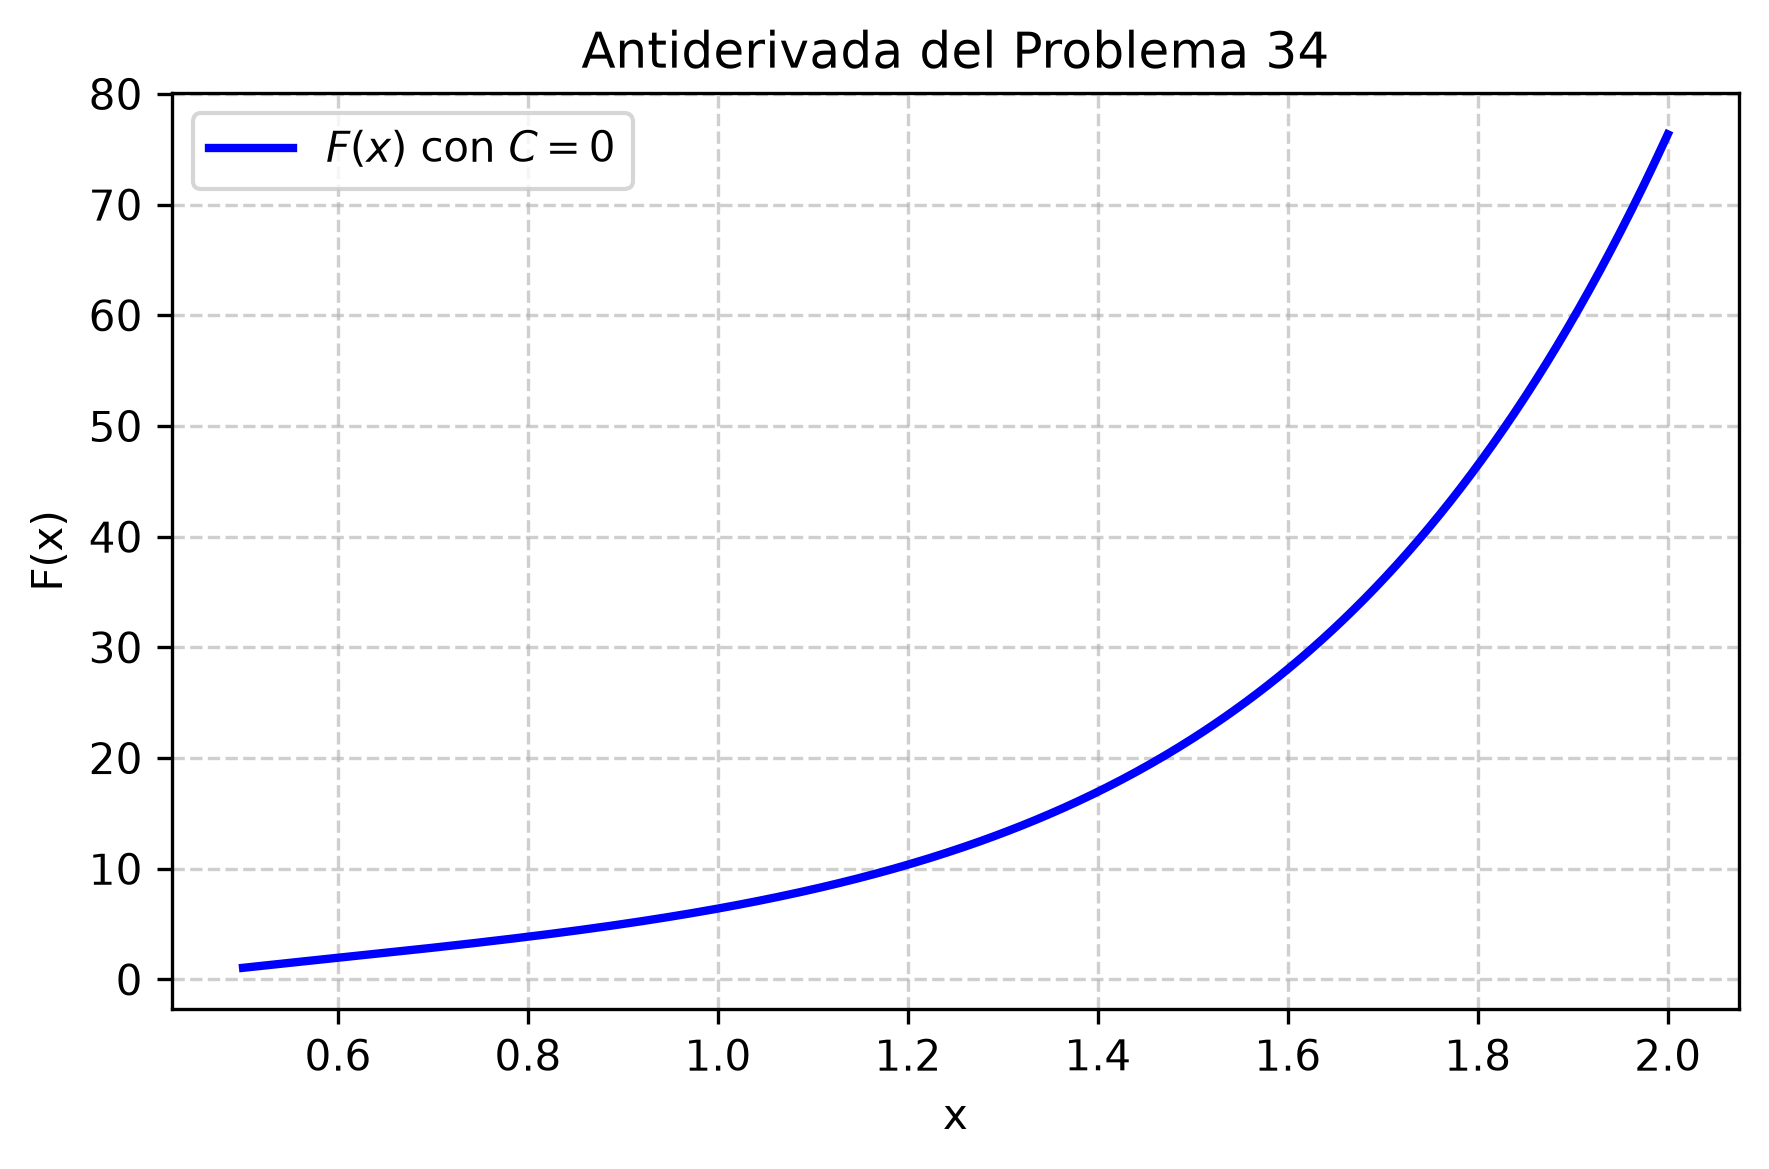
\includegraphics[width=\columnwidth]{semana_05/graficas/SEM05_P34_grafica.png}
	\caption{Representación gráfica de $f(x)$ y su antiderivada $F(x)$ evaluada para la constante de integración $C = 0$ (Problema 34).}
	\label{fig:problema34}
\end{figure}
